\section{Additional results, tables and figures}
\label{app:extra}

This appendix holds results that the main text summarizes in a sentence (\Cref{app:extra-controlled,app:extra-frozen,app:extra-lora}) and the tables and figures that support it (\Cref{app:extra-tables}).

\subsection{Controlled studies in detail (Section~\ref{sec:controlled})}
\label{app:extra-controlled}

\paragraph{Candidate selection (experiment 01).}
Nine fixed candidates compete: the true distribution, four wrong mixtures with the same mean, a permuted control and three constants.
Each criterion chooses one using 48 validation items with one, two or three sampled ratings each, over 256 independent draws; chosen candidates are scored exactly on 48 test items.
Pearson, Spearman, Kendall and scaled squared error always kept all five same-mean candidates tied, so the true distribution was in the retained set but could not be told from the four wrong ones.
This is the identification result of Section~\ref{sec:identification} at finite sample: proper losses separate same-mean forecasts, and mean-based criteria cannot.

\paragraph{Reliability is not accuracy (experiments 04 and 05).}
A judge that is wrong on 3 of 11 artifacts has relative and absolute generalizability coefficients equal to 1, the same as the oracle, with RPS $0.228$ against $0.117$.
Variance components are not useless: restricted-maximum-likelihood decision-study allocation picked the best rating design in 256 of 256 simulated replications in each of two configurations, and in the first its held-out absolute error was $0.107$ lower than equal allocation (paired difference $-0.107$, 95\% interval $[-0.149,-0.065]$; negative favors the chosen design).
The two toolkits answer different questions, and our argument is about the distribution of ratings, not against psychometric tools in their own role.

\paragraph{Calibrated heads and squared error (experiments 11, 17 and 18).}
Directly minimizing squared error fixes Pearson's drift in level and scale, and a calibration head fitted after a Pearson score fixes the rest of what a scalar can fix.
In experiment 11, cross-fitting and slope regularization cut the naive calibrated head's small-sample spike (at 32 items or fewer) by about three to nine times, and squared-error training beats a constant forecast in all four scenarios at 2{,}048 items (RPS excess $0.0076$ to $0.0118$).
Yet squared-error training leaves conditional higher moments unconstrained: at 2{,}048 items it trails the validation-selected CE fit by $0.0069$ to $0.0087$ RPS excess (all intervals above zero), and its excess CE (KL to the truth) is $0.118$ to $0.197$ nats against $0.0066$ to $0.0224$ nats.
End-to-end CE strictly dominates whenever the disagreement varies across items (scenarios A and B).
In experiment 17, a flexible calibrator on the \emph{true} mean matches or beats end-to-end CE in all four scenarios from 512 items, so a single number is not a bottleneck when it is the right number; with a score learned by Pearson training the gap closes in scenarios B, C and D but not in A (excess $+0.0052$ RPS at 2{,}048 items), because a correlation-trained score carries almost no information about spread when the mean barely moves.
Experiment 18 draws the line: a Pearson score followed by a calibrated affine head beats CE-trained judges at 128 items and above when the spread is a function of the mean (head wins 14 of 18 cells at 512 items), and loses when the spread varies independently of it (CE wins 13 of 18 cells, and all nine cells of scenario A).

\paragraph{Rater severity (experiment 15).}
On the 75 expert-rated theorem artifacts, rater offsets are about $0.1$ rating points and explain about 2\% of within-artifact variance (interval includes zero), and removing them leaves the best judge and the RPS ranking unchanged (Kendall $\tau\ge0.995$).
Item signal dominates, so severity does not explain the comparisons in the main text.

\subsection{Frozen judges in detail (Section~\ref{sec:frozen})}
\label{app:extra-frozen}

\paragraph{Five frontier judges on student homework (experiments 21 and 26).}
Two graders each scored 160 student answers to 67 questions in one University of North Texas computer-science course~\citep{mohler2011learning}; each fold holds out one whole 16-answer homework assignment and the comparison unit is the assignment (ten units).
For experiment 21 the two models were Qwen3.5-9B and Claude Sonnet 5; experiment 26 adds the five frontier judges of experiment 28 on the identical prompts.
CE-fit has lower held-out RPS than Pearson-fit in all 35 judge-by-budget cells, and the preregistered descending test (one-sided level 0.01, from 256 ratings down) passes for GPT-6 Astra and Kimi K3 down to 8 ratings and fails at 256 for the other three, whose Pearson fits are close to their CE fits (\Cref{tab:exp26}).
At 4 ratings, two distinct answers each graded twice, CE is not significantly better for four of five judges.
Qwen3.5-9B passed the test at every tested budget from 4 ratings, with test RPS $0.1548$ for the CE fit against $0.2263$ for the Pearson fit at 4 ratings, whereas Claude Sonnet 5 never passed the descending test: at 256 ratings its two fits chose the same setting in 1{,}981 of 2{,}000 draws.
For Qwen, the training grade histogram beat the CE-calibrated judge at all seven budgets, and at 256 ratings its Pearson fit had the higher held-out correlation ($0.620$ against $0.556$) while predicting a mean grade of $2.79$ for a human mean of $4.31$: the metric the objectives optimize reversed which fit looked better.

\paragraph{Public benchmarks where the judge is weaker (experiment 23).}
Direct selection by CE beat direct selection by Pearson at the largest budget on KonIQ-10k image quality~\citep{hosu2020koniq}, on dialogue ratings and on MovieLens, but not on SummEval, and the margin over strong controls is small or absent in all four.
On KonIQ-10k, with seven image indicators as the judge input, a CE fit beat raw Pearson and uniform on held-out RPS from 12 ratings (24 when the training sample is resampled as well); no tested budget from 6 to 6{,}144 ratings cleared all four controls, and a Pearson score calibrated into grade probabilities scored best at the largest budget (RPS $0.0922$ against $0.1068$ for the CE fit).
On SummEval factual consistency~\citep{fabbri2021summeval} with archived GPT-4 probabilities, CE never cleared raw Pearson and uniform from 6 to 768 ratings: at 768 ratings the CE fit selected the uniform forecast (RPS $0.2837$) while the Pearson fit scored RPS $0.1436$ and CE $1.9335$ nats against $1.6094$, and a calibrated Pearson score reached RPS $0.0543$.
On dialogue ratings (Topical-Chat and PersonaChat; 24 held-out contexts per track; 180 to 216 training grades), a calibrated Pearson-selected score had the lower RPS than a calibrated CE-selected score in all three exploratory tracks (test RPS of the calibrated Pearson judge minus test RPS of the calibrated CE judge: $-0.0133$, $-0.0092$, $-0.0026$; negative favors Pearson).
On MovieLens no budget from 6 to 768 ratings beat both Pearson and uniform, and a training histogram and a calibrated Pearson score each beat direct CE in 64 of 64 draws at 768 ratings.
The consistent lesson is that the distributional calibration step carries the gain, and that without a strong forecast distribution to start from, a histogram of the training ratings is a hard baseline.

\paragraph{Retrospective theorem judges (75 VeriBench artifacts).}
The earliest human-rating evidence is 75 theorem artifacts, 25 tasks, 19 families and 195 expert ratings, reused by experiments 02, 09, 10, 12, 14, 16, 18, 19 and 20, so these are one body of evidence and not independent replications.
Matched CE-trained and Pearson-trained mixtures of five cached judges (experiment 02) gave a test CE of the CE-trained mixture minus the test CE of the Pearson-trained mixture of $-0.260$ nats (95\% task-family bootstrap interval $[-1.458,+0.198]$; negative favors the CE-trained mixture); the interval includes zero, so the data do not establish an advantage.
Test RPS was $0.139$ for the CE-trained mixture, $0.144$ for the Pearson-trained mixture and $0.187$ for the constant forecast.
Later studies on the same ratings found CE and RPS mixtures better than the Pearson mixture at every training size (test RPS of the Pearson-trained mixture minus that of the CE-trained mixture: $+0.048$ to $+0.090$ on a 44-judge pool, significant in 8 of 8 settings, and $+0.003$ to $+0.019$ on the five-judge pool, significant at 4 and 8 training tasks only; experiment 18), CE heads better than Pearson heads from 7 training families on closed 15- and 59-judge pools ($+0.035$ to $+0.058$ RPS; experiment 20), and, for frontier judges, a Native-15 mixture with Pearson-trained minus CE-trained test RPS of $+0.0775$ (interval $[+0.0437,+0.1135]$; experiment 10).
Asking judges for a six-category probability output instead of three scalar votes lowered held-out CE from $3.480$ to $1.629$ nats for open models and from $5.49$ to $1.416$ nats for frontier models (experiments 09 and 10).
Selecting a \emph{single} judge from a pool depends on the pool.
For the 44 historical scalar-vote judges, selection by Pearson was as good as or better than selection by CE (never significantly worse, and significantly better at 8, 12 and 16 training tasks in experiment 18 and at every size in experiment 20, by $0.030$ to $0.033$ RPS), whereas for pools of native-probability judges selection by CE won by $0.011$ to $0.063$ RPS in the closed native-probability 15, the open-weight 39 and the combined 59 judges (experiment 20; nine of nine intervals exclude zero; test RPS of the Pearson-selected minus the CE-selected judge, positive favors CE selection).
Selecting by RPS did no better than selecting by CE or correlation (experiment 16).
Choosing among whole judges that differ mainly in ranking quality calls for a ranking criterion, while fitting or selecting a distribution is where CE helps.

\begin{table}[h]
\caption{\textbf{Five frontier judges on 160 homework answers at 256 training ratings (two per answer), experiment 26.}
Held-out test RPS, 0--1, lower is better; Uncal.: raw judge; Train hist.: smoothed training grade histogram; Diff.: test RPS of the Pearson-fit judge minus test RPS of the CE-fit judge (positive favors CE-fit).
Test unit: ten held-out homework assignments (16 answers each), 200 training draws per assignment; the last row is the six-grade uniform forecast.
The last column is the smallest budget down to which the one-sided level-0.01 descending test passes from 256.
Both fits search the same 27 calibration settings exhaustively on the training ratings.
\textbf{Takeaway:} CE-fit is ahead of Pearson-fit for every judge, and clears the formal test for two.}
\label{tab:exp26}
\centering\scriptsize
\setlength{\tabcolsep}{3pt}
\begin{tabular}{lrrrrrl}
\toprule
Judge & Uncal. & Train hist. & CE-fit & Pearson-fit & Diff. & Test passes down to \\
\midrule
GPT-6 Astra & 0.0858 & 0.1049 & \textbf{0.0660} & 0.0843 & +0.0183 & 8 \\
Claude Opus 5.5 & 0.0788 & 0.1049 & \textbf{0.0639} & 0.0675 & +0.0037 & none (fails at 256) \\
Kimi K3 & 0.0899 & 0.1049 & \textbf{0.0712} & 0.0996 & +0.0284 & 8 \\
GLM 5.3 & 0.1027 & 0.1049 & \textbf{0.0757} & 0.0952 & +0.0195 & none (fails at 256) \\
DeepSeek V4.1 Flash & 0.1176 & 0.1049 & \textbf{0.0827} & 0.0867 & +0.0040 & none (fails at 256) \\
\midrule
Uniform over six grades & \multicolumn{6}{l}{0.2497} \\
\bottomrule
\end{tabular}

\end{table}

\subsection{LoRA judges after calibration (Section~\ref{sec:lora})}
\label{app:extra-lora}

On HelpSteer2 the larger studies agree with the pooled result (\Cref{fig:lora-hs2}).
In experiment 24 (Qwen3-4B), calibrated CE LoRA reaches RPS $0.15200$ at 2{,}048 ratings against $0.15309$ for calibrated Pearson LoRA, a difference of $+0.0011$ (conditional 95\% interval $[+0.0002,+0.0020]$, crossed interval $[-0.0003,+0.0025]$), and CE wins 9 of 10 matched draws.
In experiment 25A, up to 8{,}192 ratings and 20 draws, the calibrated difference is $+0.0001$ (conditional interval $[-0.0008,+0.0010]$) and no budget gives a sustained win.
In experiment 25B (Llama-3.1-8B) calibrated Pearson LoRA has the lower point-estimate RPS at five of the tested budgets (32, 64, 128, 256 and 2{,}048 ratings), $-0.0011$ at 2{,}048 (conditional interval $[-0.0023,+0.0001]$).
Calibrated CE LoRA at 8{,}192 ratings reaches RPS $0.15080$, only $0.0051$ above the human leave-one-vote-out reference, and beats the unmodified base judge calibrated on all 8{,}192 labels ($0.15481$) by $+0.0040$ (interval $[+0.0019,+0.0061]$).
A $(K+2)$-parameter logit calibration recovers shape that a one-dimensional calibration misses for the Pearson-trained judge in three of seven setups (ChaosNLI-Qwen with one and five ratings per item, $+0.0013$ and $+0.0037$; HelpSteer2, $+0.0007$) and in none of the others.
In the one-dimensional calibration a sustained conditional advantage appears in alphaNLI from 16 ratings, ChaosNLI-Qwen from 32 ratings with one rating per item and from 320 with five, and HelpSteer2 from 2{,}048; the logit calibration adds ChaosNLI-Llama.

\begin{figure}[h]
\centering
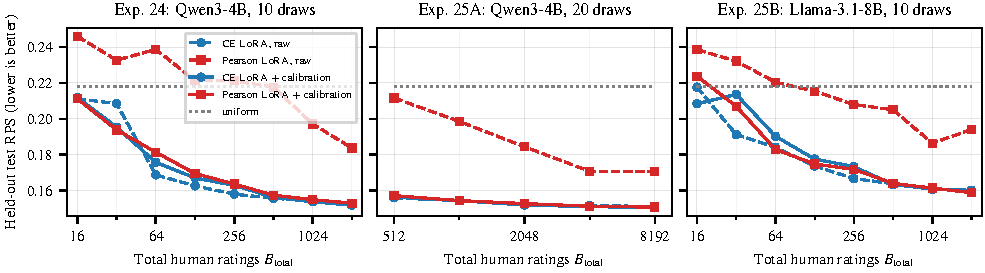
\includegraphics[width=\textwidth]{figures/fig_lora_helpsteer2.pdf}
\caption{\textbf{LoRA judges on HelpSteer2 helpfulness: raw versus calibrated forecasts.}
Vertical axis: held-out test RPS (0--1; lower is better); horizontal axis: total human ratings $B_{\mathrm{total}}$ split among training, validation and calibration.
Dashed: raw forecasts; solid: after an identical 7-parameter post-hoc calibration; blue: CE-trained; red: Pearson-trained; dotted: uniform.
Test data: 1{,}038 held-out responses from 519 held-out prompts; panels: experiment 24 (Qwen3-4B, 10 matched draws), experiment 25A (Qwen3-4B, up to 8{,}192 ratings, 20 draws) and experiment 25B (Llama-3.1-8B, 10 draws).
Human reference, leave-one-vote-out RPS: $0.14567$.
Both objectives use one optimizer, one schedule and the validation-RPS checkpoint rule; the correlation objective is not convex, so its curve reflects this optimizer, start and budget.
\textbf{Takeaway:} CE training is far better raw, but after an identical calibration the two objectives are statistically indistinguishable.}
\label{fig:lora-hs2}
\end{figure}

\subsection{Tables and figures that support the main text}
\label{app:extra-tables}

\Cref{tab:exp29} and \Cref{tab:scaling} give the numbers behind \Cref{fig:exp29} and \Cref{fig:scaling}; \Cref{fig:exp28-five} to \Cref{fig:ratings-needed} show curves that the main text summarizes in words.

\begin{table*}[t]
\caption{\textbf{Four LoRA objectives at the largest budget (experiment 29).}
Held-out test RPS of the raw forecasts (0--1; lower is better) of LoRA judges trained with CE, RPS, MSE or Pearson correlation on $B$ total human ratings, one rating per item except where noted; Qwen3-4B-Instruct-2507 or Llama-3.1-8B-Instruct; ten nested training draws per budget.
``Pearson$-$CE'' is the test RPS of the Pearson-trained judge minus the test RPS of the CE-trained judge on the same held-out items; positive favors the CE-trained judge.
The band is a two-way crossed simultaneous max-$t$ 95\% band over budgets, from 4{,}000 paired cluster-bootstrap draws that resample training draws and held-out units together.
Every judge is trained by AdamW with a validation-RPS checkpoint; the Pearson objective is not convex, so the Pearson-trained row reflects this optimizer, start and budget.
$^{\ast}$The CE and Pearson HelpSteer2 runs are those of experiment 24; the RPS and MSE runs were added in experiment 29 on the same bundle and draws.
\textbf{Takeaway:} the Pearson-trained judge is worse than the CE-trained judge in all seven setups, and the interval excludes zero in each.}
\label{tab:exp29}
\centering\scriptsize
\begin{tabular}{lrrrrrrl}
\toprule
LoRA setup & $B$ & CE & RPS & MSE & Pearson & Pearson$-$CE & Crossed 95\% band \\
\midrule
ChaosNLI, Qwen3-4B & 2048 & 0.1490 & \textbf{0.1481} & 0.1521 & 0.1622 & +0.0132 & [+0.0063, +0.0202] \\
ChaosNLI, Llama-3.1-8B & 2048 & 0.1555 & \textbf{0.1548} & 0.1580 & 0.1898 & +0.0344 & [+0.0193, +0.0494] \\
ChaosNLI, 5/item, Qwen3-4B & 1280 & \textbf{0.1530} & 0.1560 & 0.1646 & 0.1910 & +0.0379 & [+0.0216, +0.0543] \\
alphaNLI ($K{=}2$), Qwen3-4B & 1024 & \textbf{0.1862} & 0.1873 & 0.1866 & 0.2082 & +0.0220 & [+0.0117, +0.0322] \\
DICES, Qwen3-4B & 1024 & \textbf{0.2088} & 0.2101 & 0.2638 & 0.2849 & +0.0761 & [+0.0572, +0.0950] \\
DICES, Llama-3.1-8B & 1024 & \textbf{0.2060} & 0.2061 & 0.2666 & 0.2505 & +0.0445 & [+0.0191, +0.0700] \\
HelpSteer2$^{\ast}$, Qwen3-4B & 2048 & \textbf{0.1521} & 0.1527 & 0.1827 & 0.1838 & +0.0316 & [+0.0187, +0.0445] \\
\bottomrule
\end{tabular}

\end{table*}

\begin{table*}[t]
\caption{\textbf{Scaling-law fits and verdicts (experiment 31).}
Held-out test RPS (0--1; lower is better) at the largest number of human ratings $N_{\max}$ tested, for the CE-fit (or CE-trained) and the Pearson-fit (or Pearson-trained) judge; frozen-judge panels are means over five frontier judges with one rating per item, and LoRA panels are raw forecasts with ten draws per budget.
The CE-fit floor and exponent $b$ come from the weighted fit of Equation~\eqref{eq:scaling} with percentile 95\% intervals from 2{,}000 parametric bootstrap draws.
``Floor not identified'' means the floor's interval is wider than the curve's range, and ``poor power-law fit'' that the root-mean-square residual exceeds 10\% of the range.
Judges are chosen as in \Cref{fig:scaling}; exhaustive search for the head, AdamW with a validation checkpoint for LoRA.
\textbf{Takeaway:} every CE curve has a fitted exponent between $0.33$ and $0.89$, while no Pearson curve in RPS is a power law.}
\label{tab:scaling}
\centering\scriptsize
\setlength{\tabcolsep}{3pt}
\begin{tabular}{lrrrccl}
\toprule
Panel (held-out test RPS) & $N_{\max}$ & CE-fit at $N_{\max}$ & Pearson-fit at $N_{\max}$ & CE-fit floor [95\%] & CE-fit $b$ [95\%] & Pearson-fit curve (experiment 31 verdict) \\
\midrule
Exp.\ 28, ChaosNLI SNLI & 256 & 0.115 & 0.134 & 0.105 [0.000, 0.118] & 0.33 [0.04, 0.86] & slow decline, floor not identified \\
Exp.\ 28, ChaosNLI MNLI-m & 256 & 0.163 & 0.185 & 0.160 [0.147, 0.165] & 0.64 [0.28, 1.09] & slow decline, floor not identified \\
Exp.\ 28, alphaNLI (two classes) & 256 & 0.120 & 0.125 & 0.115 [0.000, 0.126] & 0.54 [0.05, 1.64] & slow decline, floor not identified \\
Exp.\ 28, DICES-350 & 256 & 0.226 & 0.276 & 0.221 [0.180, 0.231] & 0.60 [0.18, 1.13] & slow decline, floor not identified \\
Exp.\ 28, DICES-990 & 256 & 0.198 & 0.261 & 0.192 [0.159, 0.201] & 0.58 [0.21, 0.99] & flat \\
Exp.\ 29, ChaosNLI, Qwen3-4B & 2048 & 0.149 & 0.162 & 0.148 [0.146, 0.149] & 0.89 [0.76, 0.99] & slow decline, floor not identified \\
Exp.\ 29, ChaosNLI, Llama-3.1-8B & 2048 & 0.155 & 0.190 & 0.151 [0.146, 0.154] & 0.64 [0.49, 0.78] & poor power-law fit \\
Exp.\ 29, alphaNLI, Qwen3-4B & 1024 & 0.186 & 0.208 & 0.179 [0.117, 0.184] & 0.56 [0.13, 0.92] & poor power-law fit \\
Exp.\ 29, DICES, Qwen3-4B & 1024 & 0.209 & 0.285 & 0.204 [0.196, 0.208] & 0.71 [0.46, 0.96] & flat \\
Exp.\ 29, DICES, Llama-3.1-8B & 1024 & 0.206 & 0.251 & 0.203 [0.194, 0.206] & 0.89 [0.50, 1.29] & poor power-law fit \\
Exp.\ 29, HelpSteer2, Qwen3-4B & 2048 & 0.152 & 0.184 & 0.151 [0.149, 0.152] & 0.76 [0.64, 0.89] & slow decline, floor not identified \\
\bottomrule
\end{tabular}

\end{table*}

\begin{figure}[t]
\centering
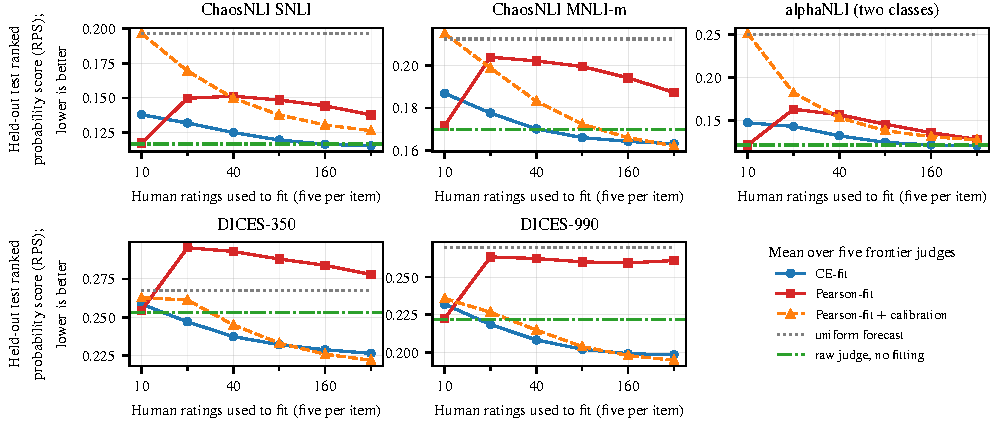
\includegraphics[width=0.92\textwidth]{figures/fig_exp28_five_per_item.pdf}
\caption{\textbf{Frozen frontier judges with five ratings per item (experiment 28).}
Vertical axis: held-out test RPS (0--1; lower is better), mean over five frontier judges; horizontal axis: human ratings used to fit, 10 to 320 (2 to 64 items with five ratings each; log scale).
Data: ChaosNLI SNLI (600 items), MNLI-matched (600), alphaNLI (400; two classes), DICES-350 (350) and DICES-990 (400 items); each held-out item is scored against all of its collected labels.
CE-fit minimizes, and Pearson-fit maximizes, its objective on the training ratings over 27 calibration settings of the judge's own probabilities, by exhaustive search; Pearson-fit + calibration follows the Pearson-chosen setting with four quantile-bin category frequencies (0.5 pseudo-count) fitted on the same training ratings.
Each point averages 200 draws; no interval is drawn here, and the break-even budgets of \Cref{tab:exp28} come from simultaneous one-sided 97.5\% bounds.
\textbf{Takeaway:} in every set the Pearson-fit curve is worse at 20 ratings than at 10 and stays above the raw judge at every larger budget, while the CE-fit curve falls at every step.}
\label{fig:exp28-five}
\end{figure}

\begin{figure}[t]
\centering
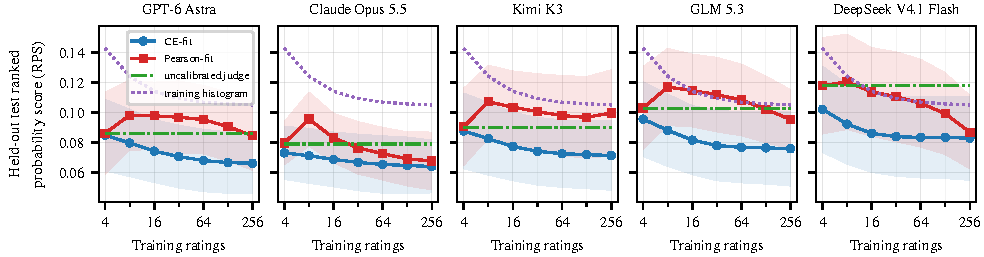
\includegraphics[width=\textwidth]{figures/fig_exp26_per_judge.pdf}
\caption{\textbf{Five frontier judges on fresh homework (experiment 26).}
Vertical axis: held-out test RPS (0--1; lower is better) on 16 held-out answers per fold, scored against two grader scores each; horizontal axis: training ratings, 4 to 256, two per answer (log scale).
Data: 160 short answers of 67 questions in ten homework folds, each fold held out once; the lines are means over folds and 200 training draws.
Shaded bands are 95\% two-sided overlap-adjusted $t$ intervals over the ten folds (standard deviation times $\sqrt{1/10+1/9}$, 9 degrees of freedom) for the CE-fit and Pearson-fit judges.
CE-fit and Pearson-fit choose among 27 calibration settings of each judge's six grade probabilities by exhaustive search on the training ratings.
\textbf{Takeaway:} the CE-fit curve lies below the Pearson-fit curve in all 35 judge-by-budget cells, but the bands overlap everywhere, so the figure supports the ranking and does not identify any law.}
\label{fig:exp26}
\end{figure}

\begin{figure}[t]
\centering
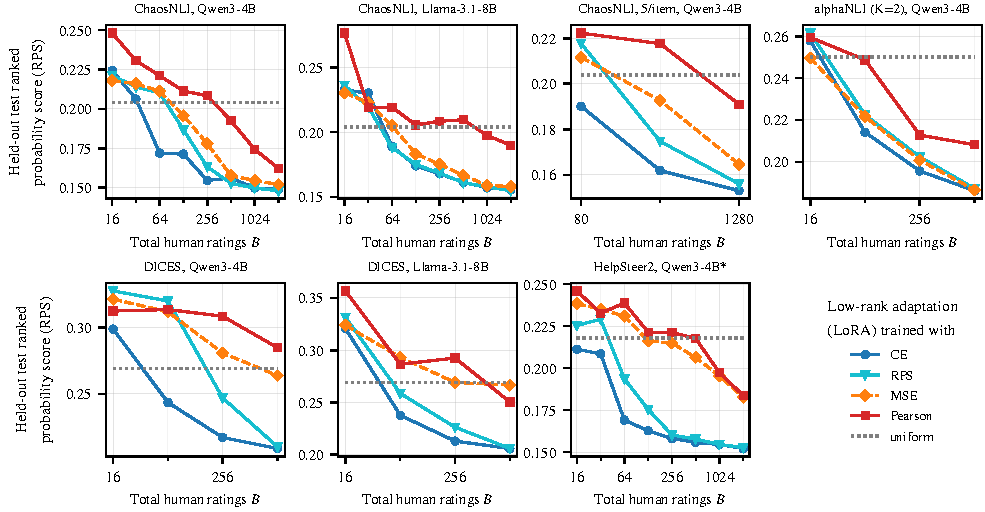
\includegraphics[width=\textwidth]{figures/fig_exp29_curves.pdf}
\caption{\textbf{Learning curves of four LoRA objectives (experiment 29).}
Vertical axis: held-out test RPS (0--1; lower is better) of raw forecasts; horizontal axis: total human ratings $B$ used for training (log scale), one rating per item unless the panel says five per item.
LoRA of Qwen3-4B-Instruct-2507 or Llama-3.1-8B-Instruct on ChaosNLI, alphaNLI (two classes), DICES and HelpSteer2 (CE and Pearson from experiment 24); each point is a mean over ten nested training draws, and no band is drawn (bands for the largest budget are in \Cref{tab:exp29}).
Each objective uses one optimizer, one schedule and the same validation-RPS checkpoint rule; the correlation objective is not convex, so it reflects this optimizer, start and budget.
\textbf{Takeaway:} CE and RPS training track each other, squared error follows them at $K=2$ and falls behind at $K\ge3$, and the Pearson-trained curve lies above the CE curve at nearly every budget.}
\label{fig:exp29-curves}
\end{figure}

\begin{figure}[t]
\centering
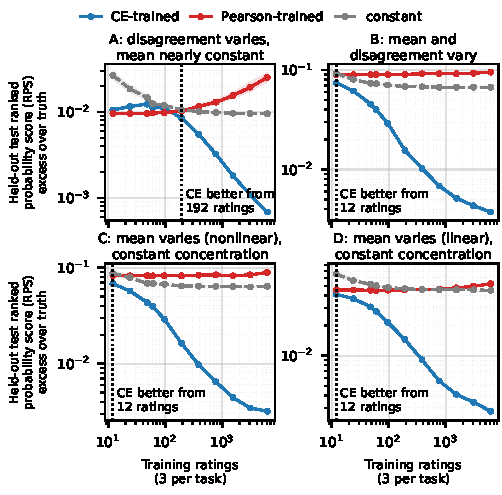
\includegraphics[width=0.56\textwidth]{figures/fig_ratings_needed.pdf}
\caption{\textbf{Ratings needed in four synthetic scenarios (experiment 08).}
Vertical axis: held-out test RPS excess over the true distribution, that is the RPS of the judge's forecast minus the RPS of the true conditional distribution on 500 fresh tasks (lower is better; log scale); horizontal axis: training ratings, three per task.
Targets are beta-binomial distributions over six ratings: A has an almost constant mean and varying disagreement, B a nonlinear mean and varying disagreement, C a nonlinear mean and constant concentration, D a linear mean and constant concentration.
The judge is a softmax over a linear map of 13 features, trained by L-BFGS-B (400 iterations) from the training histogram with a fixed ridge; the CE objective is convex and the Pearson objective is not, so the Pearson curve reflects this optimizer and start.
Lines are means over 100 seeds with 95\% percentile bootstrap bands (10{,}000 draws); the dotted line marks the smallest budget from which the paired difference (Pearson-trained minus CE-trained) has a lower bound above zero at every larger budget.
\textbf{Takeaway:} where the mean carries the signal (B, C, D) the CE-trained judge wins from 12 ratings; only in A, where the mean says little, the CE-trained judge needs 192 ratings.}
\label{fig:ratings-needed}
\end{figure}

\clearpage
